
\begin{frame}

% Use the codeblock environment to create a code block
%\begin{fancycode}{https://github.com/}{testtext}
%# Your code snippet here
%\lstinputlisting[style=kkcodestyle, basicstyle=\tiny, language=Python]{Figures/mtc/rhs_sample.py}
%\begin{lstlisting}[style=kkcodestyle, basicstyle=\tiny, language=Python]
%def hello_world():
%   print("Hello, world!")
%\end{lstlisting}
%\end{fancycode}
%\codeblockwithtab{\lstinputlisting[style=kkcodestyle, basicstyle=\tiny, language=Python]{Figures/mtc/rhs_sample.py}{https://github.com}{testtext}}
%\codeblockwithtab{\href{https://github.com}}{testtext} % You can add other content to your slide here
%\blockwithtab{testtxt}{testlnk}
\begin{tikzpicture}
        \node at (0,0) {\snippetbox{Figures/mtc/rhs_sample.py}{\href{https://github.com}{testlnk}}};
\end{tikzpicture}

\end{frame}


\begin{frame}\frametitle{M-to-N Procedure Outline}
\begin{minipage}{0.49\textwidth}
\begin{itemize}
\item Generate the input mesh (\textit{gmsh} or built-in \textit{meshmode})
\item Create the target decompositions $M$,$N$
  \begin{itemize}
  \item Creates required mapping files
  \item Run \textit{meshdist} part to $M$, $N$ ranks
  \end{itemize}
\item Run \mirgecom{} on $M$ ranks
\begin{itemize}
\item Example: Reading pre-generated mesh
\item Generates $M$ restart files per dump
\end{itemize}
\item Perform M-to-N transfer with \textit{redist}
\item Restart \mirgecom{} on $N$ ranks -or-
\item Post-processing/viz for $N$ ranks
\end{itemize}
\end{minipage}
\hfill
\begin{minipage}{.49\textwidth}
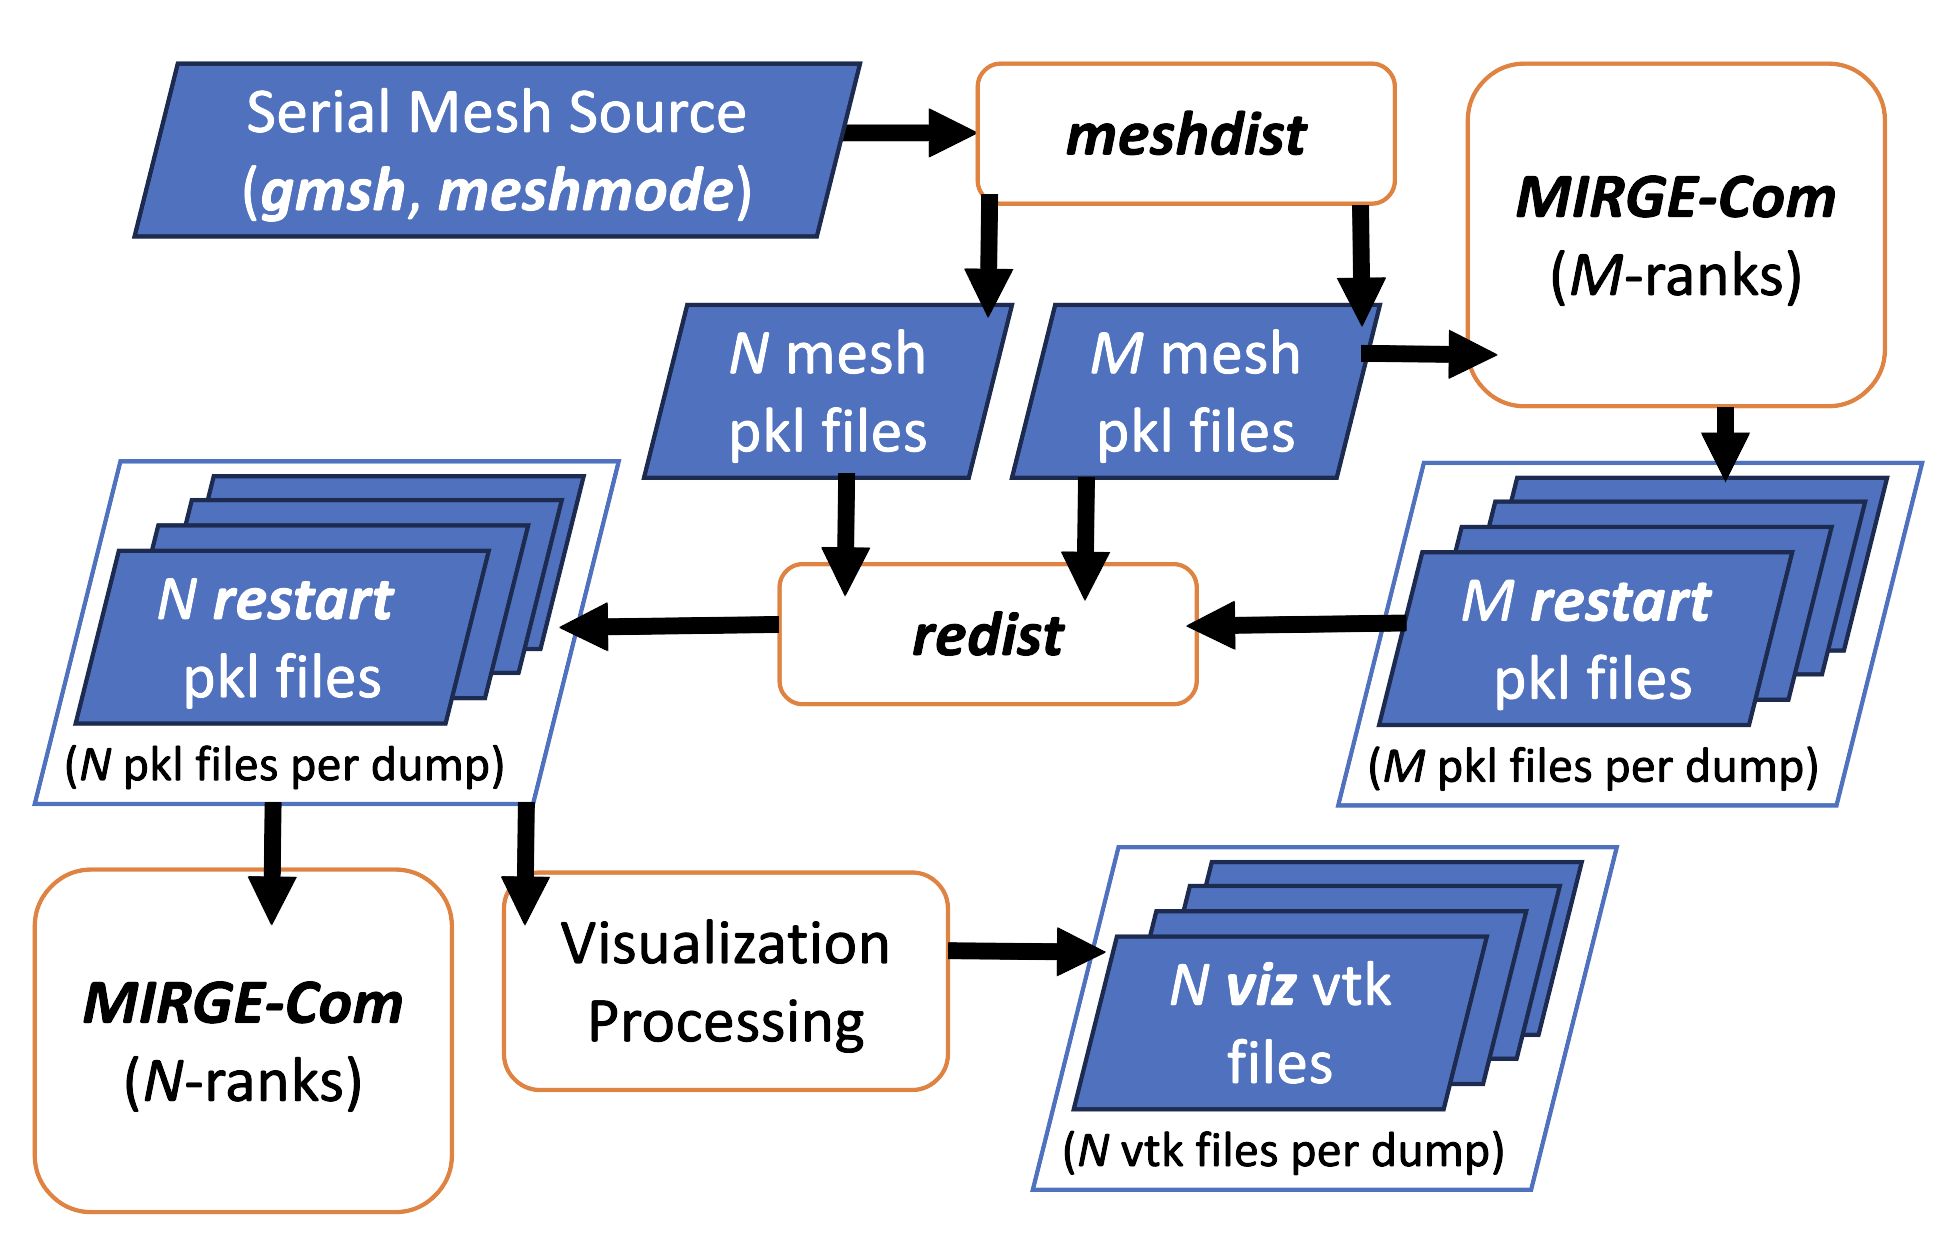
\includegraphics[width=\textwidth]{Figures/mtc/redist_data_flow_full.png}
\end{minipage}
\end{frame}

\begin{frame}\frametitle{M-to-N Procedure Outline}
\begin{minipage}{0.49\textwidth}
\begin{itemize}
\item Generate the input mesh (\textit{gmsh} or built-in \textit{meshmode})
\color{lightgray}
\item Create the target decompositions $M$,$N$
  \begin{itemize}
  \color{lightgray}
  \item Creates required mapping files
  \item Run \textit{meshdist} part to $M$, $N$ ranks
  \end{itemize}
\item Run \mirgecom{} on $M$ ranks
\begin{itemize}
\color{lightgray}
\item Example: Reading pre-generated mesh
\item Generates $M$ restart files per dump
\end{itemize}
\item Perform M-to-N transfer with \textit{redist}
\item Restart \mirgecom{} on $N$ ranks -or-
\item Post-processing/viz for $N$ ranks
\end{itemize}
\end{minipage}
\hfill
\begin{minipage}{.49\textwidth}
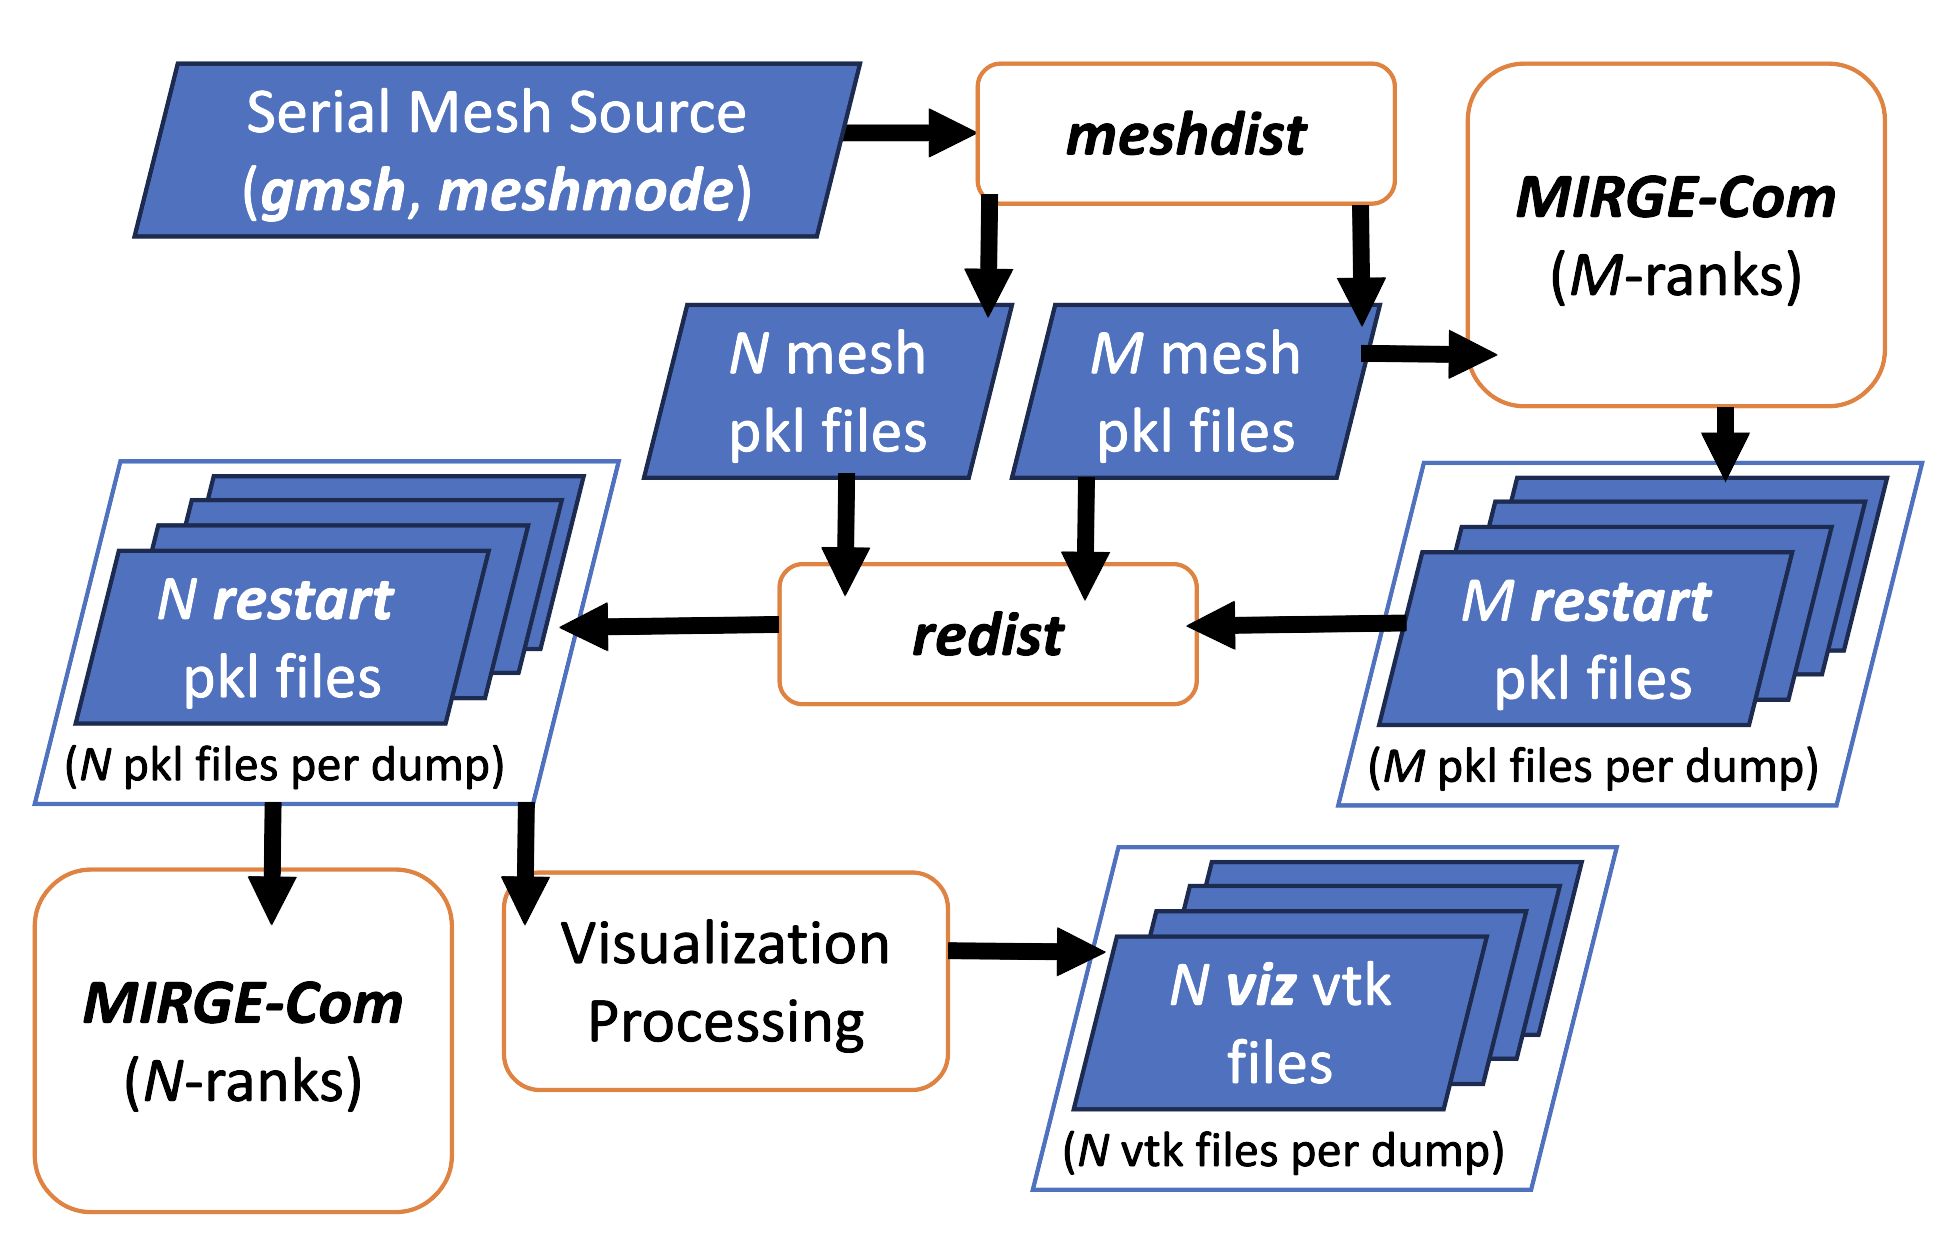
\includegraphics[width=\textwidth]{Figures/mtc/redist_data_flow_full.png}
\end{minipage}
\end{frame}


% ========= Simple examples of grid generation and import from gmsh ==============
\begin{frame}[fragile]\frametitle{Generate a Mesh with Meshmode \prj{\tiny}{M.~Smith}}

\begin{minipage}{0.5\textwidth}
\begin{itemize}
\item Mesh generator functions in \textit{meshmode} can be used to create simple
  geometries
\end{itemize}
\end{minipage}

\begin{tikzpicture}[overlay,remember picture]
\node(code)at([xshift=-1.3in,yshift=-0.5in]current page.center){
  \begin{minipage}{0.5\textwidth}
    \begin{lstlisting}[style=mintedlike,basicstyle=\mintedlikebasicstyle{\footnotesize}]
  from meshmode.mesh.generation import \
      generate_regular_rect_mesh
  mesh = generate_regular_rect_mesh(
      a=(-L/2, -L/2),
      b=(L/2, L/2),
      n=16,
      boundary_tag_to_face={
          "LeftRight": ["-x", "+x"],
          "BottomTop": ["-y", "+y"]})
    \end{lstlisting}
  \end{minipage}
};
\end{tikzpicture}
\hfill
\begin{minipage}{0.5\textwidth}

\begin{tikzpicture}[scale=0.4]
    % Grid
    \draw[step=1, thin, black] (0,0) grid (16,10);
    \draw[thick] (0,0) rectangle (16,10);
\end{tikzpicture}
\end{minipage}

\end{frame}

\begin{frame}[fragile]\frametitle{Generate Multivolume Mesh with Meshmode}

\begin{minipage}{0.5\textwidth}
\begin{itemize}
\item Creation of multi-volume mesh with \textit{meshmode}
\end{itemize}
\end{minipage}

\begin{tikzpicture}[overlay,remember picture]
\node(code)at([xshift=-1.3in,yshift=-0.5in]current page.center){
  \begin{minipage}{0.5\textwidth}
    \begin{lstlisting}[style=mintedlike,basicstyle=\mintedlikebasicstyle{\footnotesize}]
  from meshmode.mesh.generation import \
      generate_regular_rect_mesh
  mesh = generate_regular_rect_mesh(
      a=(-L/2, -L/2),
      b=(L/2, L/2),
      n=16,
      boundary_tag_to_face={
          "LeftRight": ["-x", "+x"],
          "BottomTop": ["-y", "+y"]})
  x_avg = np.sum(x, axis=1)/x.shape[1]
  tag_to_elements = {
      "Vol1": np.where(x_avg < vol1_loc)[0],
      "Vol2": np.where(x_avg > vol1_loc)[0]}
    \end{lstlisting}
  \end{minipage}
};
\end{tikzpicture}
\hfill
\begin{minipage}{0.5\textwidth}
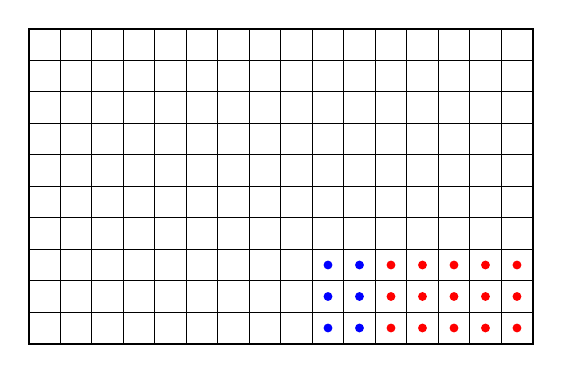
\begin{tikzpicture}[scale=0.4]
    % Grid
    \draw[step=1, thin, black] (0,0) grid (16,10);
    \draw[thick] (0,0) rectangle (16,10);
    % Red subregion
    \foreach \i in {11, 12, 13, 14, 15} {
        \foreach \j in {0, 1, 2} {
            \fill[red] (\i+0.5, \j+0.5) circle (4pt);
        }
    }
    
    % Blue subregion
    \foreach \i in {9, 10} {
        \foreach \j in {0, 1, 2} {
            \fill[blue] (\i+0.5, \j+0.5) circle (4pt);
        }
    }
\end{tikzpicture}
\begin{tikzpicture}[overlay, remember picture, scale=0.3]
% Legend Box
  \begin{scope}[xshift=-20.8cm, yshift=16.8cm]
    \draw[thick] (-1,0.5) rectangle (6,-3); % Adjusted the top border of the box
   
    \fill[blue] (0,-0.5) circle (6pt); % Blue dot
    \node[align=left] at (3,-0.5) {Volume 1}; % Moved the label to the right
     
    \fill[red] (0,-2) circle (6pt);  % Red dot
    \node[align=left] at (3,-2) {Volume 2}; % Moved the label to the right
  \end{scope}
\end{tikzpicture}
\end{minipage}

\end{frame}


\begin{frame}[fragile]\frametitle{Generate a Tensor Product Mesh with Meshmode}

\begin{minipage}{0.5\textwidth}
\begin{itemize}
\item Creation of tensor product element mesh with \textit{meshmode}
\end{itemize}
\end{minipage}

\begin{tikzpicture}[overlay,remember picture]
\node(code)at([xshift=-1.3in,yshift=-0.5in]current page.center){
  \begin{minipage}{0.5\textwidth}
    \begin{lstlisting}[style=mintedlike,basicstyle=\mintedlikebasicstyle{\footnotesize}]
  from meshmode.mesh import \
      TensorProductElementGroup
  from meshmode.mesh.generation import \
      generate_regular_rect_mesh
  mesh = generate_regular_rect_mesh(
      a=(-L/2, -L/2),
      b=(L/2, L/2),
      n=16,
      boundary_tag_to_face={
          "LeftRight": ["-x", "+x"],
          "BottomTop": ["-y", "+y"]},
      group_cls=TensorProductElementGroup)
    \end{lstlisting}
  \end{minipage}
};
\end{tikzpicture}
\hfill
\begin{minipage}{0.5\textwidth}

\begin{tikzpicture}[scale=0.4]
    % Grid
    \draw[step=1, thin, black] (0,0) grid (16,10);
    \draw[thick] (0,0) rectangle (16,10);
\end{tikzpicture}
\end{minipage}

\end{frame}


\begin{frame}[fragile]\frametitle{Import a Gmsh Mesh \prj{\tiny}{M.~Smith}}
\vspace{-0.9in}

\begin{minipage}{0.5\textwidth}
\begin{itemize}
\item Otherwise, use \textit{Gmsh} to generate meshes from CAD
\item Multi-volume supported natively in \textit{Gmsh}
\end{itemize}
\end{minipage}

\begin{tikzpicture}[overlay,remember picture]
\node(code)at([xshift=-1.3in,yshift=-0.5in]current page.center){
  \begin{minipage}{0.5\textwidth}
    \begin{lstlisting}[style=mintedlike,basicstyle=\mintedlikebasicstyle{\footnotesize}]
def get_mesh_data():
  from meshmode.mesh.io import read_gmsh
  mesh, tag_to_elements = \
    read_gmsh(
       mesh_filename, force_ambient_dim=dim,
       return_tag_to_elements_map=True)
  volume_to_tags = {
     "fluid": ["fluid"],
     "wall":  ["wall_insert", "wall_surround"]
  }
  return mesh, tag_to_elements, volume_to_tags
  \end{lstlisting}
  \end{minipage}
};
\end{tikzpicture}

\begin{tikzpicture}[overlay,remember picture]
\node(anchor)at([xshift=1.6in]current page.center){};
\node(nozzlemesh)at([yshift=0.8in]anchor.center){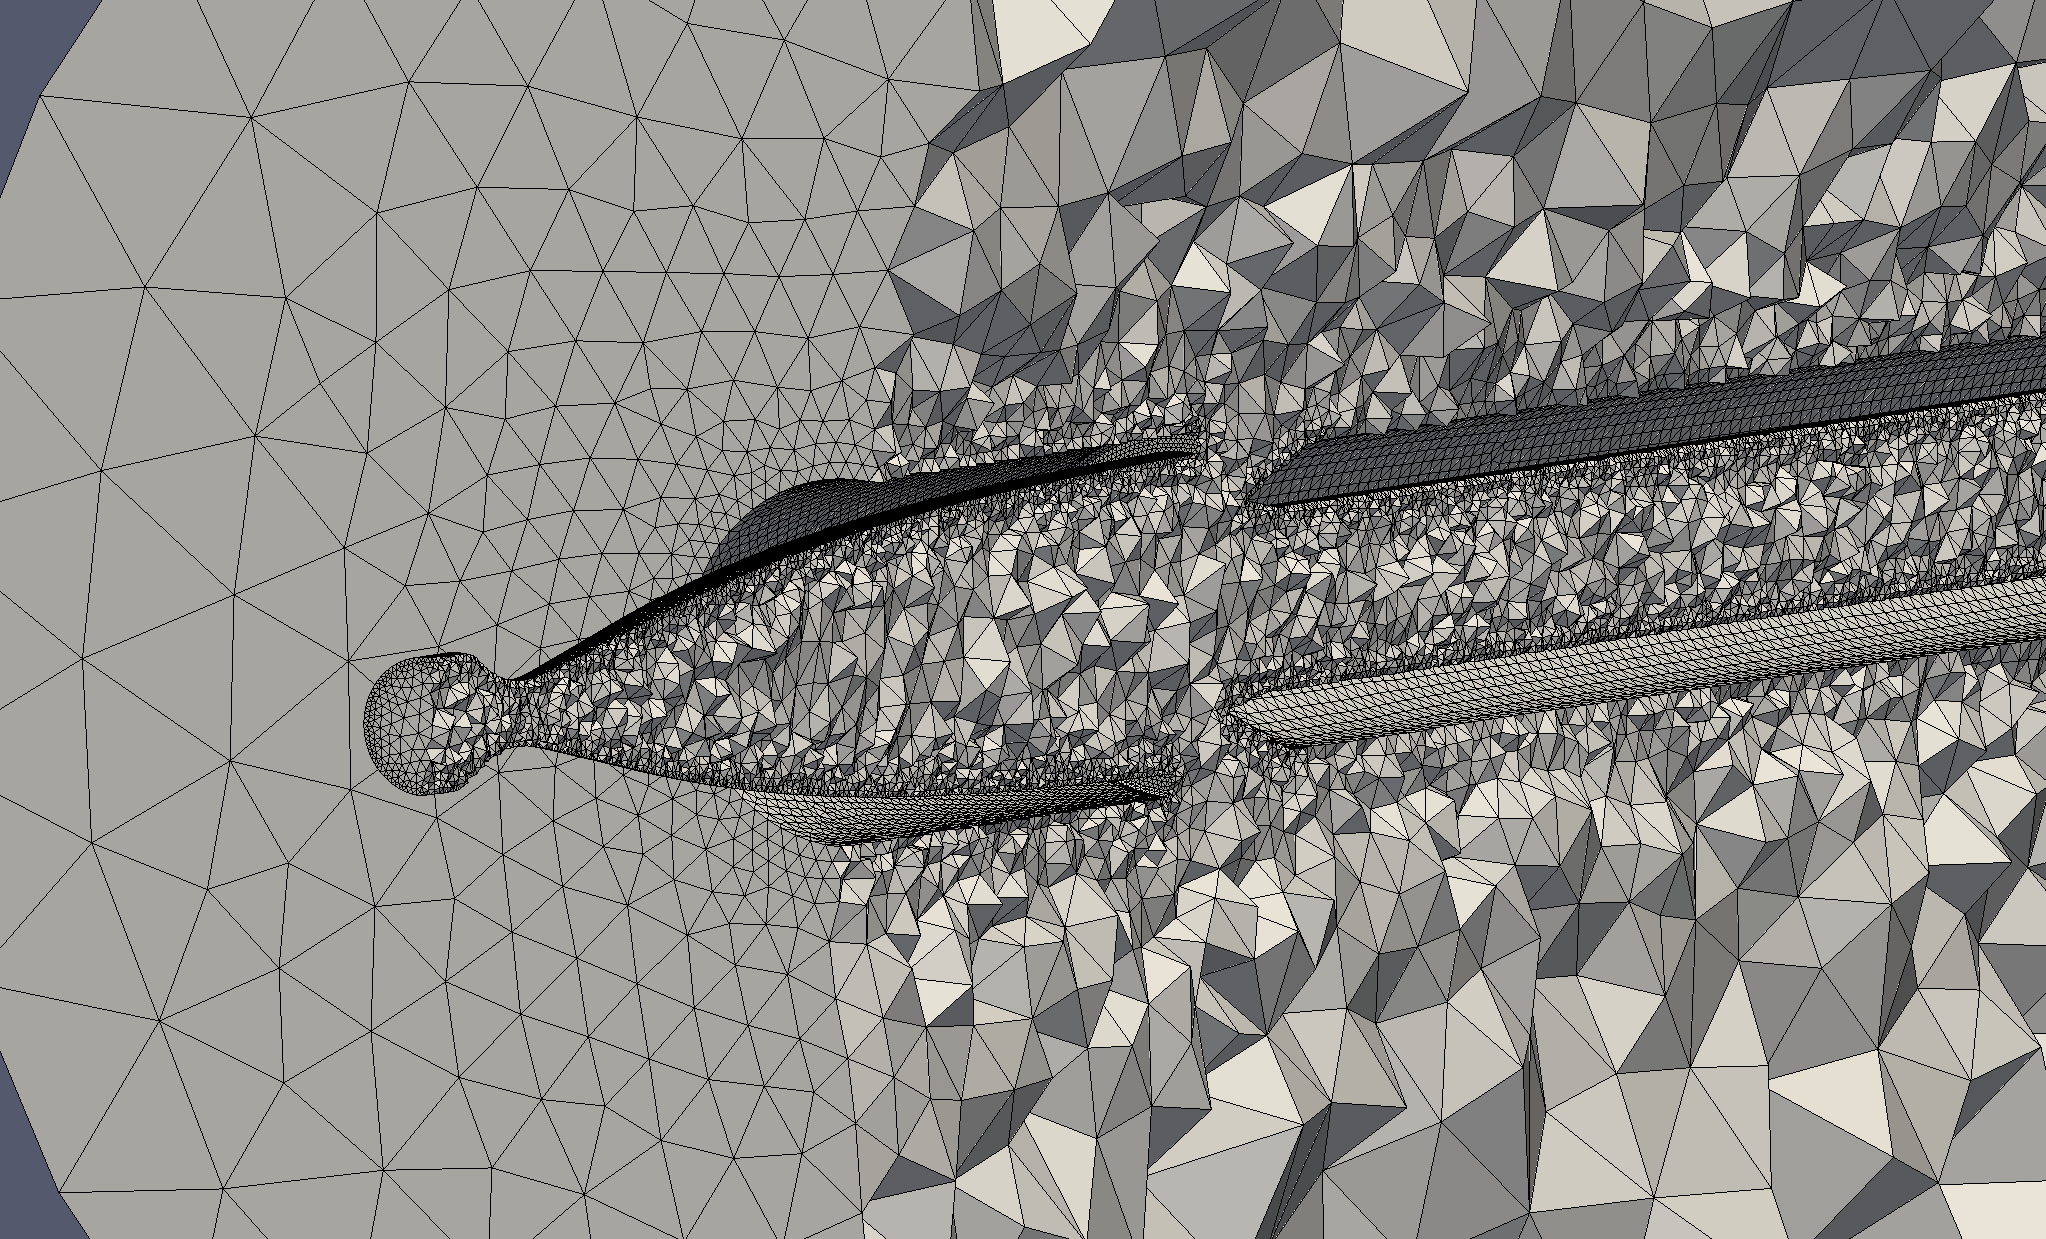
\includegraphics[width=0.4\textwidth]{Figures/mtc/nozzle_mesh.png}};
\node(y3mesh)at([yshift=-0.9in]anchor.center){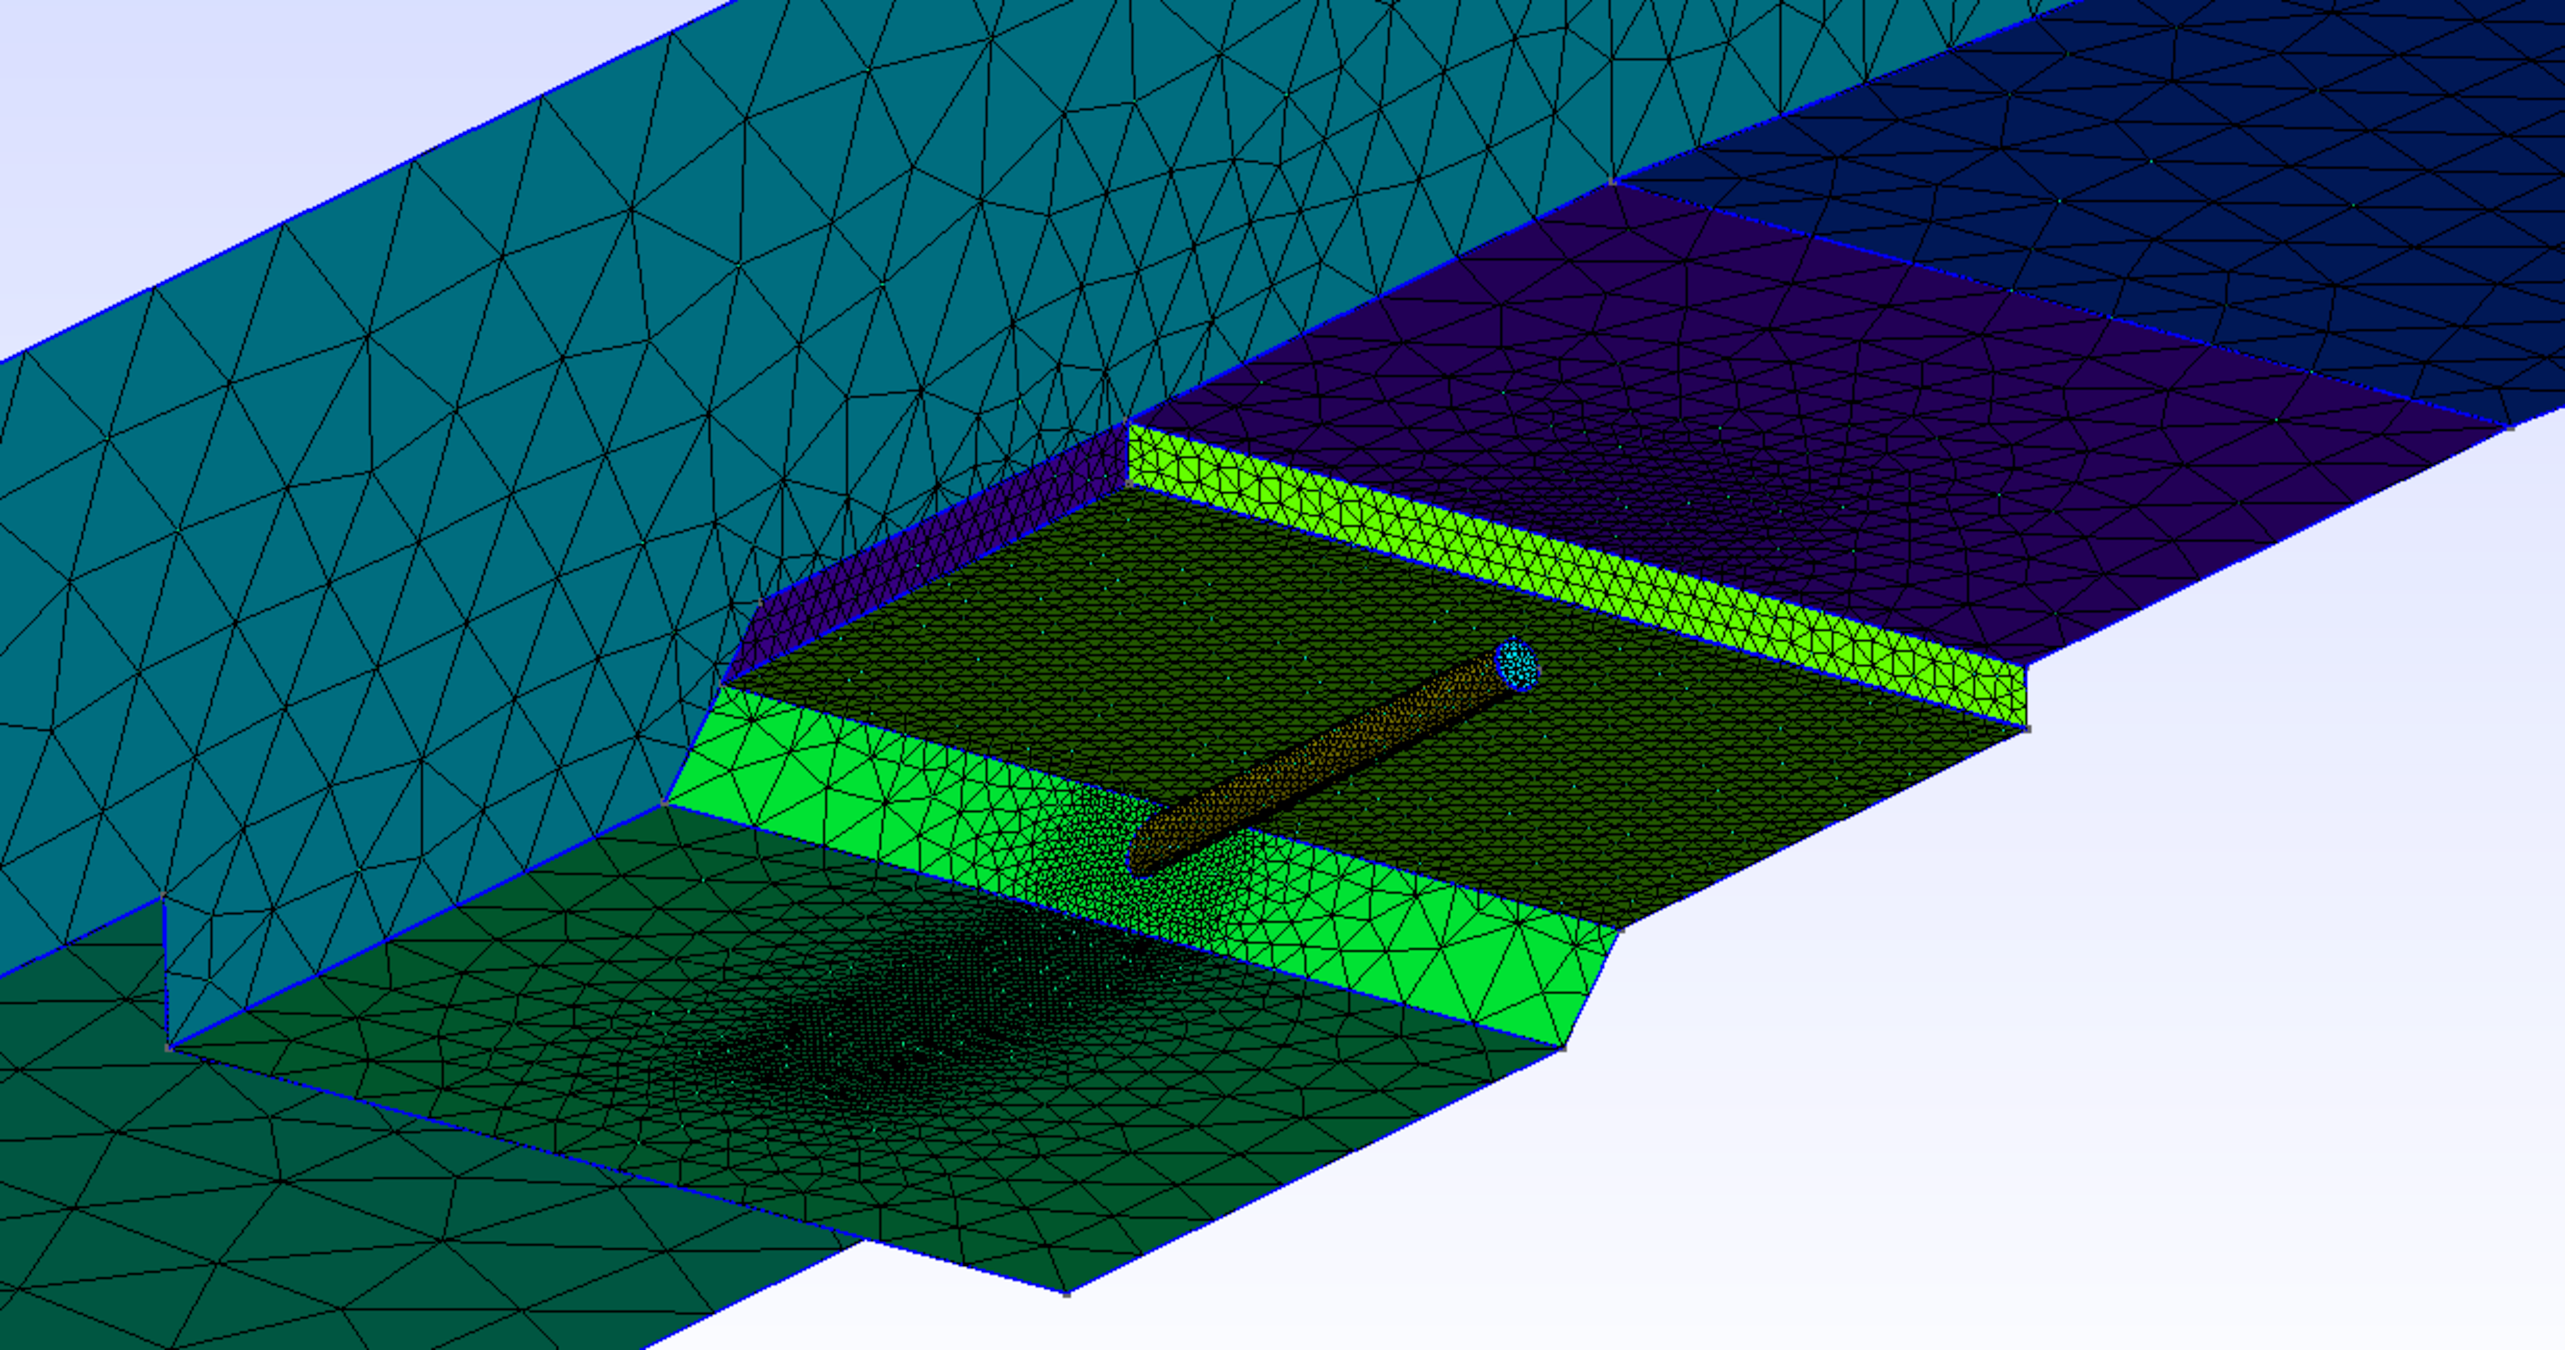
\includegraphics[width=0.4\textwidth]{Figures/mtc/3d_mesh_cavity.pdf}};
\node(ref)at([xshift=-0.1in]y3mesh.south){\prj{\tiny}{M.~Anderson, 02}};
\end{tikzpicture}

\end{frame}
% ================================================================================

% Regardless of mesh source/generator, mesh is in this general form:
\begin{frame}\frametitle{Global Mesh: Input}
\vspace{-20pt}
\begin{minipage}[t][0.3\textheight][t]{\textwidth}
\begin{itemize}
\item Typically coming from gmsh or other software
\item Total number of elements in the global mesh: $N_E$
\item Globally numbered elements: $E_n = [0, 1, 2,..., N_E)$
\end{itemize}
\end{minipage}
%\hfill
\vfill
\begin{tikzpicture}[overlay, remember picture, scale=0.4]
\begin{scope}[shift={(10, -5)}]
    % Grid
    \draw[step=1, thin, black] (0,0) grid (16,10);
    \draw[thick] (0,0) rectangle (16,10);
    
    \def\flatteneddata{
        0, 1, 3, 6, 10, 15, 21, 28, 36, 45, 55, 65, 75, 85, 95, 105, 
        2, 4 , 7, 11, 16, 22, 29, 37, 46, 56, 66, 76, 86, 96, 106, 115, 
        5, 8, 1  2, 17, 23, 30, 38, 47, 57, 67, 77, 87, 97, 107, 116, 124, 
        9, 13, 18, 24, 31, 39, 48, 58, 68, 78, 88, 98, 108, 117, 125, 132, 
        14, 19, 25, 32, 40, 49, 59, 69, 79, 89, 99, 109, 118, 126, 133, 139, 
        20, 26, 33, 41, 50, 60, 70, 80, 90, 100, 110, 119, 127, 134, 140, 145, 
        27, 34, 42, 51, 61, 71, 81, 91, 101, 111, 120, 128, 135, 141, 146, 150, 
        35, 43, 52, 62, 72, 82, 92, 102, 112, 121, 129, 136, 142, 147, 151, 154, 
        44, 53, 63, 73, 83, 93, 103, 113, 122, 130, 137, 143, 148, 152, 155, 157, 
        54, 64, 74, 84, 94, 104, 114, 123, 131, 138, 144, 149, 153, 156, 158, 159
    }
    
    \xdef\mycount{0}
    \foreach \value in \flatteneddata {
        % Calculate x and y coordinates based on the mycount
        \pgfmathtruncatemacro\x{\mycount - 16 * (int(\mycount/16))}
        \pgfmathtruncatemacro\y{int(\mycount/16)}
        
        \node at (\x+0.5, 9.5-\y) {\tiny \value};
        
        \pgfmathtruncatemacro\incrementedcount{\mycount + 1}
        \xdef\mycount{\incrementedcount}
    }
\end{scope}
\end{tikzpicture}

\end{frame}


\begin{frame}\frametitle{\textit{meshdist}: \mirgecom{} Mesh Partitioning Utility}
\begin{itemize}
\item Creates an $M$-decomposition of an input mesh
\item Mirrors built-in decomposition, except:
  \begin{itemize}
  \item Writes mapping files required by m-to-n
    \begin{itemize}
    \item Decomp map: $r_m[E_N]$  (maps global element id $E_n$ to MPI rank $r_m$)
    \item PartID map: $P[E_N]$ (maps global element id to PartID $P$)
    \item PartID is (volume, rank) pair
    \end{itemize}
  \item Writes $M$-decomposed mesh into pkl file per rank
  \end{itemize}
\item Divides work across $P$ processors (max used $= M$)
\begin{itemize}
\item Each \textit{meshdist} rank locally handles $M / P$ mesh partitions
\item Reads input mesh on all ranks
\item Global partitioning on all ranks
\item Local meshmode datastructures for locally-handled $M$-parts
\item Writes locally-handled $M$-parts to pkl
\end{itemize}
\end{itemize}
\end{frame}

\begin{frame}\frametitle{Mesh and Solution I/O in \mirgecom{}}
\begin{multicols}{2}
  \begin{itemize}
    % \setlength{\itemsep}{0.2in}
    %\item MIRGE-Com Overview
    \item Serial mesh processing
    \begin{itemize}
    \item Mesh source (gmsh[multivol], meshmode generator, etc)
    \item Meshmode datastructure ingest
    \end{itemize}
    \item Partitioning and distribution
    \begin{itemize}
    \item Global partitioning (1dpart, metis, whatever)
    \item Meshmode datastructure ingest
    \item Mesh distribution
    \begin{itemize}
    \item built-in
    \item pre-processing
    \end{itemize}
    \end{itemize}
    \item Create DG Discretization
    \begin{itemize}
    \item Element group factories
    \item Multivolume considerations
    \item DOFArrays
    \end{itemize}
    \item Simulation Data
    \begin{itemize}
    \item Restart (pkl file / process)
    \item Visualization  (vtk file / process)
    \end{itemize}
    \item M-to-N Restart
    \begin{itemize}
    \item inter-decomp element index mapping
    \item Mapping solution-to-volume
    \end{itemize}
  \end{itemize}
  \end{multicols}
%\end{minipage}
%\hfill
%\begin{minipage}[T]{0.45\textwidth}
%  \centering
%  \tikzstyle{c_mirgecom}=[draw=myOrange, line width=0.5mm]
%  \softwaredeps%
%\end{minipage}
%  \url{https://github.com/illinois-ceesd/mirgecom/}
\end{frame}

\begin{frame}\frametitle{Mesh Sources}
\begin{itemize}
\item meshmode
\item gmsh
\end{itemize}
\end{frame}

\begin{frame}\frametitle{M-to-N Restarts}
\begin{itemize}
\item M-to-N refers to when we want to change the number of \textit{partitions} in the \textit{global mesh} \textit{decomposition}
\begin{itemize}
  \item \textbf{global mesh}: The finite-element discretized domain (elements)   
  \item \textbf{partition}: The rank-specific part of a decomposed mesh
  \item \textbf{decomposition}: A set of partitions that cover the global mesh
\end{itemize}
\end{itemize}
\end{frame}

\begin{frame}{TikZ Positioning}
    \begin{tikzpicture}[remember picture, overlay]
    % Absolute positioning
    \node at (current page.center) (center) {Center};
    \begin{scope}[shift={(8cm, -8cm)}]

        % Relative positioning
        \node[above=2cm of center] (above) {Above};
        \node[below=2cm of center] (below) {Below};
        \node[left=2cm of center] (left) {Left};
        \node[right=2cm of center] (right) {Right};

        % Connecting nodes
        \draw[->, red] (center) -- (above);
        \draw[->, blue] (center) -- (below);
        \draw[->, green] (center) -- (left);
        \draw[->, orange] (center) -- (right);
    \end{scope}
    \end{tikzpicture}
\end{frame}

\begin{frame}\frametitle{Global Mesh: Input}
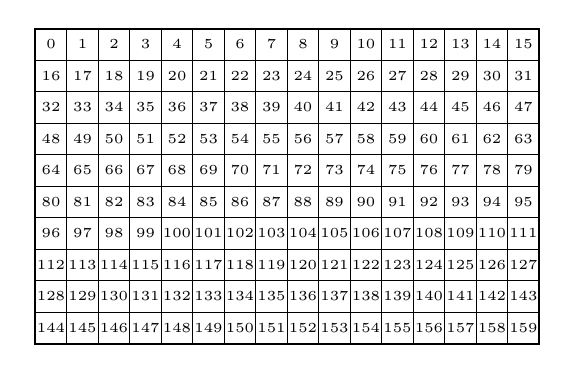
\begin{tikzpicture}[scale=0.4]
    \begin{scope}
    % Grid
    \draw[step=1, thin, black] (0,0) grid (16,10);
    \draw[thick] (0,0) rectangle (16,10);
    
    % Numbering
    \foreach \y in {0,...,9} {
        \foreach \x in {0,...,15} {
            \pgfmathsetmacro{\num}{int(\y*16+\x)}
            \node at (\x+0.5, 9.5-\y) {\tiny \num};
        }
    }
\end{scope}
\end{tikzpicture}
\end{frame}

\begin{frame}\frametitle{Global Mesh: Input}
\vspace{-20pt}
\begin{minipage}[t][0.3\textheight][t]{\textwidth}
\begin{itemize}
\item Typically coming from gmsh or other software
\item Total number of elements in the global mesh: $N_E$
\item Globally numbered elements: $E_n = [0, 1, 2,..., N_E)$
\end{itemize}
\end{minipage}
%\hfill
\vfill
\begin{tikzpicture}[overlay, remember picture, scale=0.4]
\begin{scope}[shift={(10, -5)}]
    % Grid
    \draw[step=1, thin, black] (0,0) grid (16,10);
    \draw[thick] (0,0) rectangle (16,10);

    % Numbering
    \foreach \y in {0,...,9} {
        \foreach \x in {0,...,15} {
            \pgfmathsetmacro{\num}{int(\y*16+\x)}
            \node at (\x+0.5, 9.5-\y) {\tiny \num};
        }
    }
\end{scope}
\end{tikzpicture}
%\vfill
%\hfill
\end{frame}


\begin{frame}\frametitle{Global Mesh: Input}
\vspace{-20pt}
\begin{minipage}[t][0.3\textheight][t]{\textwidth}
\begin{itemize}
\item Typically coming from gmsh or other software
\item Total number of elements in the global mesh: $N_E$
\item Globally numbered elements: $E_n = [0, 1, 2,..., N_E)$
\end{itemize}
\end{minipage}
%\hfill
\vfill
\begin{tikzpicture}[overlay, remember picture, scale=0.4]
\begin{scope}[shift={(10, -5)}]
    % Grid
    \draw[step=1, thin, black] (0,0) grid (16,10);
    \draw[thick] (0,0) rectangle (16,10);
\end{scope}
\end{tikzpicture}
%\vfill
%\hfill
\end{frame}



\begin{frame}\frametitle{Global Mesh: Input}
\begin{itemize}
\item Global (gmsh) mesh enters \mirgecom{} through serial read:
  \begin{itemize}
  \item \textit{read\_gmsh}
  \item \textit{meshmode ingest}
  \end{itemize}
\item TODO: Timing and memory usage for these stages.
\end{itemize}
\end{frame}

\begin{frame}\frametitle{Single Volume Partitioning}
\begin{minipage}[t][0.3\textheight][t]{\textwidth}
\end{minipage}
\begin{tikzpicture}[overlay, remember picture, scale=0.3]
    \node at (2cm, -15cm) (center) {};

    \begin{scope}[shift={(center)}]  % yshift=-10cm]

    % Grid
    \draw[step=1, thin, black] (0,0) grid (16,10);
    \draw[thick] (0,0) rectangle (16,10);

    \begin{scope}[xshift=30cm]
    % Partition 0
    \draw[step=1, thin, black] (0,0) grid (4,10);
    \draw[thick] (0,0) rectangle (4,10);
    \node[font=\bfseries, blue] at (2,9) {0};
    
    % Partition 1
    \begin{scope}[xshift=4.5cm]
        \draw[step=1, thin, black] (0,0) grid (4,10);
        \draw[thick] (0,0) rectangle (4,10);
        \node[font=\bfseries, blue] at (2,9) {1};
    \end{scope}
    
    % Partition 2 with blue and red subregions
    \begin{scope}[xshift=9cm]
        \draw[step=1, thin, black] (0,0) grid (4,10);
        \draw[thick] (0,0) rectangle (4,10);
        \node[font=\bfseries, blue] at (2,9) {2};
    \end{scope}
    
    % Partition 3 with red subregion
    \begin{scope}[xshift=13.5cm]
        \draw[step=1, thin, black] (0,0) grid (4,10);
        \draw[thick] (0,0) rectangle (4,10);
        \node[font=\bfseries, blue] at (2,9) {3};
    \end{scope}

    \end{scope}
    
    % Coordinates for arrow
    \coordinate (leftGridCenter) at (8,5);
    \coordinate (rightGridCenter) at (38,5);
    
    % Arrow with text
    \draw[->, ultra thick] (leftGridCenter) -- node[midway, fill=white, text width=3cm, align=center] {Your Text Here} (rightGridCenter);
    \end{scope}


\end{tikzpicture}
\end{frame}

\begin{frame}\frametitle{Single Volume Partitioning}
\begin{minipage}[t][0.3\textheight][t]{\textwidth}
\end{minipage}
\begin{tikzpicture}[overlay, remember picture, scale=0.3]
    \begin{scope}[yshift=-10cm]
    % Grid
    \draw[step=1, thin, black] (0,0) grid (16,10);
    \draw[thick] (0,0) rectangle (16,10);
    \end{scope}

    \begin{scope}[xshift=30cm, yshift=-10cm]
    % Partition 0
    \draw[step=1, thin, black] (0,0) grid (4,10);
    \draw[thick] (0,0) rectangle (4,10);
    \node[font=\bfseries, blue] at (2,9) {0};
    
    % Partition 1
    \begin{scope}[xshift=4.5cm]
        \draw[step=1, thin, black] (0,0) grid (4,10);
        \draw[thick] (0,0) rectangle (4,10);
        \node[font=\bfseries, blue] at (2,9) {1};
    \end{scope}
    
    % Partition 2 with blue and red subregions
    \begin{scope}[xshift=9cm]
        \draw[step=1, thin, black] (0,0) grid (4,10);
        \draw[thick] (0,0) rectangle (4,10);
        % \foreach \j in {0, 1, 2} {
        %    \fill[blue] (1.5, \j+0.5) circle (4pt);
        %    \fill[blue] (2.5, \j+0.5) circle (4pt);
        %    \fill[red] (3.5, \j+0.5) circle (4pt);
        %}
        \node[font=\bfseries, blue] at (2,9) {2};
    \end{scope}
    
    % Partition 3 with red subregion
    \begin{scope}[xshift=13.5cm]
        \draw[step=1, thin, black] (0,0) grid (4,10);
        \draw[thick] (0,0) rectangle (4,10);
        %\foreach \j in {0, 1, 2} {
        %    \fill[red] (0.5, \j+0.5) circle (4pt);
        %    \fill[red] (1.5, \j+0.5) circle (4pt);
        %    \fill[red] (2.5, \j+0.5) circle (4pt);
        %    \fill[red] (3.5, \j+0.5) circle (4pt);
        %}
        \node[font=\bfseries, blue] at (2,9) {3};
    \end{scope}
    \end{scope}
\end{tikzpicture}
\end{frame}

\begin{frame}\frametitle{M-to-N Restarts}
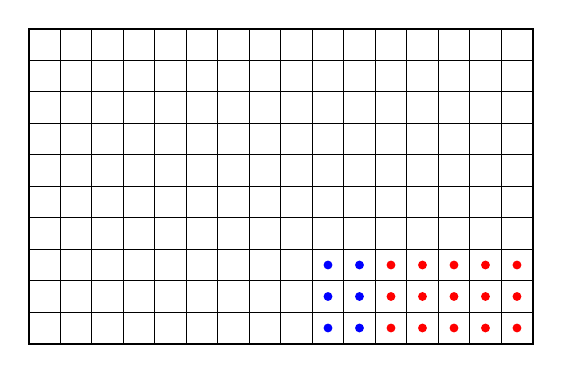
\begin{tikzpicture}[scale=0.4]
    % Grid
    \draw[step=1, thin, black] (0,0) grid (16,10);
    \draw[thick] (0,0) rectangle (16,10);
    
    % Red subregion
    \foreach \i in {11, 12, 13, 14, 15} {
        \foreach \j in {0, 1, 2} {
            \fill[red] (\i+0.5, \j+0.5) circle (4pt);
        }
    }
    
    % Blue subregion
    \foreach \i in {9, 10} {
        \foreach \j in {0, 1, 2} {
            \fill[blue] (\i+0.5, \j+0.5) circle (4pt);
        }
    }
\end{tikzpicture}
\end{frame}

\begin{frame}\frametitle{M-to-N Restarts}
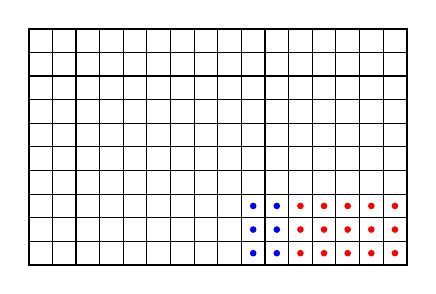
\begin{tikzpicture}[scale=0.3]
    % Grid
    \draw[step=1, thin, black] (0,0) grid (16,10);
    \draw[thick] (0,0) rectangle (16,10);
    
    % Red subregion
    \foreach \i in {11, 12, 13, 14, 15} {
        \foreach \j in {0, 1, 2} {
            \fill[red] (\i+0.5, \j+0.5) circle (4pt);
        }
    }
    
    % Blue subregion
    \foreach \i in {9, 10} {
        \foreach \j in {0, 1, 2} {
            \fill[blue] (\i+0.5, \j+0.5) circle (4pt);
        }
    }
\end{tikzpicture}
\end{frame}

\begin{frame}\frametitle{M-to-N Restarts}
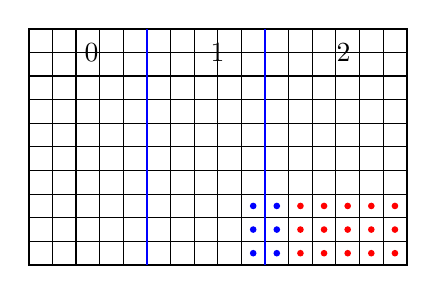
\begin{tikzpicture}[scale=0.3]
    % Grid
    \draw[step=1, thin, black] (0,0) grid (16,10);
    \draw[thick] (0,0) rectangle (16,10);
    
    % Red subregion
    \foreach \i in {11, 12, 13, 14, 15} {
        \foreach \j in {0, 1, 2} {
            \fill[red] (\i+0.5, \j+0.5) circle (4pt);
        }
    }
    
    % Blue subregion
    \foreach \i in {9, 10} {
        \foreach \j in {0, 1, 2} {
            \fill[blue] (\i+0.5, \j+0.5) circle (4pt);
        }
    }

    % Partition lines and labels for 3 partitions
    \draw[thick, blue] (5,0) -- (5,10);
    \draw[thick, blue] (10,0) -- (10,10);
    
    \node at (2.66,9) {0};
    \node at (7.99,9) {1};
    \node at (13.33,9) {2};
\end{tikzpicture}
\end{frame}

\begin{frame}\frametitle{M-to-N Restarts}
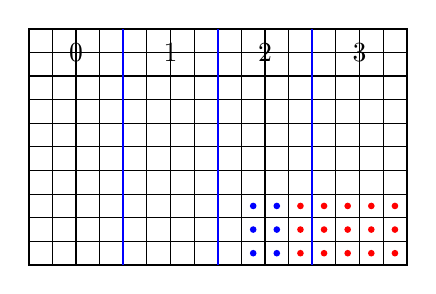
\begin{tikzpicture}[scale=0.3]
    % Grid
    \draw[step=1, thin, black] (0,0) grid (16,10);
    \draw[thick] (0,0) rectangle (16,10);
    
    % Red subregion
    \foreach \i in {11, 12, 13, 14, 15} {
        \foreach \j in {0, 1, 2} {
            \fill[red] (\i+0.5, \j+0.5) circle (4pt);
        }
    }
    
    % Blue subregion
    \foreach \i in {9, 10} {
        \foreach \j in {0, 1, 2} {
            \fill[blue] (\i+0.5, \j+0.5) circle (4pt);
        }
    }

    % Partition lines and labels
    \draw[thick, blue] (4,0) -- (4,10);
    \draw[thick, blue] (8,0) -- (8,10);
    \draw[thick, blue] (12,0) -- (12,10);

    \node at (2,9) {0};
    \node at (6,9) {1};
    \node at (10,9) {2};
    \node at (14,9) {3};
\end{tikzpicture}
\end{frame}


\begin{frame}\frametitle{M-to-N Restarts}
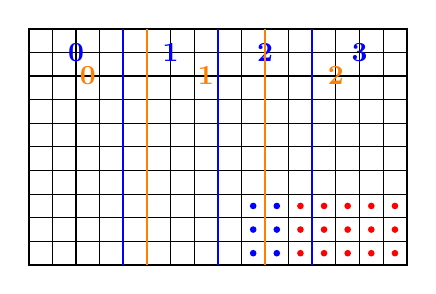
\begin{tikzpicture}[scale=0.3]
    % Grid
    \draw[step=1, thin, black] (0,0) grid (16,10);
    \draw[thick] (0,0) rectangle (16,10);
    
    % Red subregion
    \foreach \i in {11, 12, 13, 14, 15} {
        \foreach \j in {0, 1, 2} {
            \fill[red] (\i+0.5, \j+0.5) circle (4pt);
        }
    }
    
    % Blue subregion
    \foreach \i in {9, 10} {
        \foreach \j in {0, 1, 2} {
            \fill[blue] (\i+0.5, \j+0.5) circle (4pt);
        }
    }

    % Partition lines and labels for 4 partitions (in blue)
    \draw[thick, blue] (4,0) -- (4,10);
    \draw[thick, blue] (8,0) -- (8,10);
    \draw[thick, blue] (12,0) -- (12,10);
    
    \node[font=\bfseries, blue] at (2,9) {0};
    \node[font=\bfseries, blue] at (6,9) {1};
    \node[font=\bfseries, blue] at (10,9) {2};
    \node[font=\bfseries, blue] at (14,9) {3};

    % Partition lines for 3 partitions (in orange)
    \draw[thick, orange] (5,0) -- (5,10);
    \draw[thick, orange] (10,0) -- (10,10);
    
    \node[font=\bfseries, orange] at (2.5,8) {0};
    \node[font=\bfseries, orange] at (7.5,8) {1};
    \node[font=\bfseries, orange] at (13,8) {2};
\end{tikzpicture}
\end{frame}

\begin{frame}
\frametitle{M-to-N Restart}
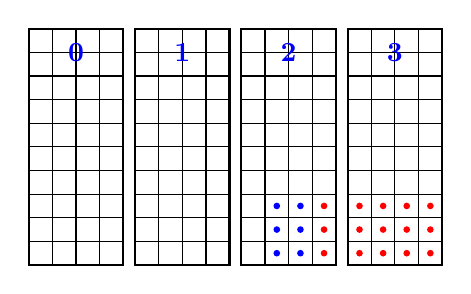
\begin{tikzpicture}[scale=0.3]

    % Partition 0
    \draw[step=1, thin, black] (0,0) grid (4,10);
    \draw[thick] (0,0) rectangle (4,10);
    \node[font=\bfseries, blue] at (2,9) {0};
    
    % Partition 1
    \begin{scope}[xshift=4.5cm]
        \draw[step=1, thin, black] (0,0) grid (4,10);
        \draw[thick] (0,0) rectangle (4,10);
        \node[font=\bfseries, blue] at (2,9) {1};
    \end{scope}
    
    % Partition 2 with blue and red subregions
    \begin{scope}[xshift=9cm]
        \draw[step=1, thin, black] (0,0) grid (4,10);
        \draw[thick] (0,0) rectangle (4,10);
        \foreach \j in {0, 1, 2} {
            \fill[blue] (1.5, \j+0.5) circle (4pt);
            \fill[blue] (2.5, \j+0.5) circle (4pt);
            \fill[red] (3.5, \j+0.5) circle (4pt);
        }
        \node[font=\bfseries, blue] at (2,9) {2};
    \end{scope}
    
    % Partition 3 with red subregion
    \begin{scope}[xshift=13.5cm]
        \draw[step=1, thin, black] (0,0) grid (4,10);
        \draw[thick] (0,0) rectangle (4,10);
        \foreach \j in {0, 1, 2} {
            \fill[red] (0.5, \j+0.5) circle (4pt);
            \fill[red] (1.5, \j+0.5) circle (4pt);
            \fill[red] (2.5, \j+0.5) circle (4pt);
            \fill[red] (3.5, \j+0.5) circle (4pt);  % added this line for the last column of red dots in partition 3
        }
        \node[font=\bfseries, blue] at (2,9) {3};
    \end{scope}
\end{tikzpicture}
\end{frame}

\begin{frame}
\frametitle{M-to-N Restart}
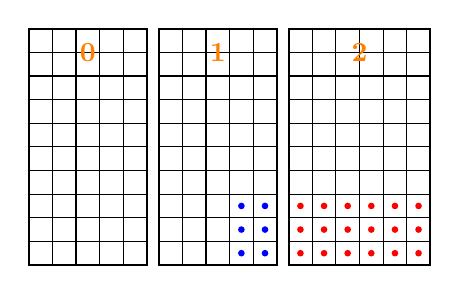
\begin{tikzpicture}[scale=0.3]

    % Partition 0
    \draw[step=1, thin, black] (0,0) grid (5,10);
    \draw[thick] (0,0) rectangle (5,10);
    \node[font=\bfseries, orange] at (2.5,9) {0};
    
    % Partition 1 with blue subregion
    \begin{scope}[xshift=5.5cm]
        \draw[step=1, thin, black] (0,0) grid (5,10);
        \draw[thick] (0,0) rectangle (5,10);
        \foreach \j in {0, 1, 2} {
            \fill[blue] (3.5, \j+0.5) circle (4pt);
            \fill[blue] (4.5, \j+0.5) circle (4pt);
        }
        \node[font=\bfseries, orange] at (2.5,9) {1};
    \end{scope}
    
    % Partition 2 with red subregion
    \begin{scope}[xshift=11cm]
        \draw[step=1, thin, black] (0,0) grid (6,10);
        \draw[thick] (0,0) rectangle (6,10);
        \foreach \j in {0, 1, 2} {
            \fill[red] (0.5, \j+0.5) circle (4pt);
            \fill[red] (1.5, \j+0.5) circle (4pt);
            \fill[red] (2.5, \j+0.5) circle (4pt);
            \fill[red] (3.5, \j+0.5) circle (4pt);
            \fill[red] (4.5, \j+0.5) circle (4pt);
            \fill[red] (5.5, \j+0.5) circle (4pt);
        }
        \node[font=\bfseries, orange] at (3,9) {2};
    \end{scope}
\end{tikzpicture}
\end{frame}

%\begin{frame}
%\frametitle{Grid without Border on Cutout}
%\begin{tikzpicture}[scale=0.3]
%
%    % Draw only the visible cells
%    \foreach \i in {0,1,2,3} {
%        \foreach \j in {3,4,...,9} {
%            \draw (\i,\j) rectangle (\i+1,\j+1);
%        }
%    }
%    \draw (0,0) rectangle (1,3);
%    \draw (0,0) rectangle (1,1);
%    \draw (0,1) rectangle (1,2);
%    \draw (0,2) rectangle (1,3);
%
%    % Adjusted border
%    \draw[thick] (0,0) -- (1,0) -- (1,3) -- (4,3) -- (4,10) -- (0,10) -- cycle;
%
%\end{tikzpicture}
%\end{frame}

\begin{frame}
\frametitle{M-to-N Restart}
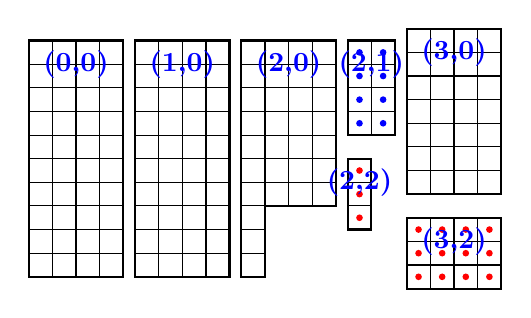
\begin{tikzpicture}[scale=0.3]

    % Partition (0,0)
    \draw[step=1, thin, black] (0,0) grid (4,10);
    \draw[thick] (0,0) rectangle (4,10);
    \node[font=\bfseries, blue] at (2,9) {(0,0)};

    % Partition (1,0)
    \begin{scope}[xshift=4.5cm]
        \draw[step=1, thin, black] (0,0) grid (4,10);
        \draw[thick] (0,0) rectangle (4,10);
        \node[font=\bfseries, blue] at (2,9) {(1,0)};
    \end{scope}

    % Partition (2,0) with the correct shape and border
    \begin{scope}[xshift=9cm]
        \foreach \i in {0,1,2,3} {
            \foreach \j in {3,4,...,9} {
                \draw (\i,\j) rectangle (\i+1,\j+1);
            }
        }
        \draw (0,0) rectangle (1,3);
        \draw (0,0) rectangle (1,1);
v        \draw (0,1) rectangle (1,2);
        \draw (0,2) rectangle (1,3);
        \draw[thick] (0,0) -- (1,0) -- (1,3) -- (4,3) -- (4,10) -- (0,10) -- cycle;
        \node[font=\bfseries, blue] at (2,9) {(2,0)};
    \end{scope}

    % Partition (2,1) with blue subregion, adjusted position
    \begin{scope}[xshift=13.5cm, yshift=6cm]
        \draw[step=1, thin, black] (0,0) grid (2,4);
        \draw[thick] (0,0) rectangle (2,4);
        \foreach \j in {0,1,2,3} {
            \fill[blue] (0.5, \j+0.5) circle (4pt);
            \fill[blue] (1.5, \j+0.5) circle (4pt);
        }
        \node[font=\bfseries, blue] at (1,3) {(2,1)};
    \end{scope}

    % Partition (2,2) with red subregion, adjusted position
    \begin{scope}[xshift=13.5cm, yshift=2cm]
        \draw[step=1, thin, black] (0,0) grid (1,3);
        \draw[thick] (0,0) rectangle (1,3);
        \foreach \j in {0,1,2} {
            \fill[red] (0.5, \j+0.5) circle (4pt);
        }
        \node[font=\bfseries, blue] at (0.5,2) {(2,2)};
    \end{scope}

    % Partition (3,0), adjusted position and dimensions
    \begin{scope}[xshift=16cm, yshift=3.5cm]
        \draw[step=1, thin, black] (0,0) grid (4,7);
        \draw[thick] (0,0) rectangle (4,7);
        \node[font=\bfseries, blue] at (2,6) {(3,0)};
    \end{scope}

    % Partition (3,2) with red subregion, adjusted position
    \begin{scope}[xshift=16cm, yshift=-0.5cm]
        \draw[step=1, thin, black] (0,0) grid (4,3);
        \draw[thick] (0,0) rectangle (4,3);
        \foreach \j in {0,1,2} {
            \fill[red] (0.5, \j+0.5) circle (4pt);
            \fill[red] (1.5, \j+0.5) circle (4pt);
            \fill[red] (2.5, \j+0.5) circle (4pt);
            \fill[red] (3.5, \j+0.5) circle (4pt);
        }
        \node[font=\bfseries, blue] at (2,2) {(3,2)};
    \end{scope}

\end{tikzpicture}
\end{frame}

\begin{frame}
\frametitle{M-to-N Restart}
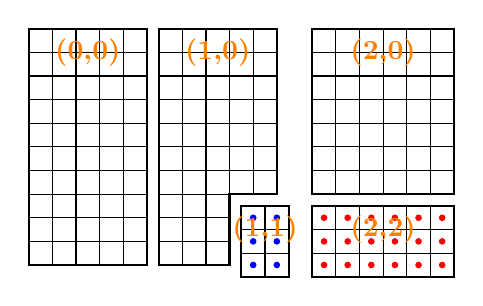
\begin{tikzpicture}[scale=0.3]

    % Partition (0,0)
    \draw[step=1, thin, black] (0,0) grid (5,10);
    \draw[thick] (0,0) rectangle (5,10);
    \node[font=\bfseries, orange] at (2.5,9) {(0,0)};

    % Partition (1,0) with the correct shape, border, and panhandle grid
    \begin{scope}[xshift=5.5cm]
        \foreach \i in {0,1,2,3,4} {
            \foreach \j in {3,4,...,9} {
                \draw (\i,\j) rectangle (\i+1,\j+1);
            }
        }
        \foreach \i in {0,1,2} {
            \foreach \j in {0,1,2} {
                \draw (\i,\j) rectangle (\i+1,\j+1);
            }
        }
        \draw[thick] (0,0) -- (3,0) -- (3,3) -- (5,3) -- (5,10) -- (0,10) -- cycle;
        \node[font=\bfseries, orange] at (2.5,9) {(1,0)};
    \end{scope}

    % Partition (1,1) with blue subregion, further adjusted position
    \begin{scope}[xshift=9cm, yshift=-0.5cm]
        \draw[step=1, thin, black] (0,0) grid (2,3);
        \draw[thick] (0,0) rectangle (2,3);
        \foreach \j in {0,1,2} {
            \fill[blue] (0.5, \j+0.5) circle (4pt);
            \fill[blue] (1.5, \j+0.5) circle (4pt);
        }
        \node[font=\bfseries, orange] at (1,2) {(1,1)};
    \end{scope}

    % Partition (2,0)
    \begin{scope}[xshift=12cm, yshift=3cm]
        \draw[step=1, thin, black] (0,0) grid (6,7);
        \draw[thick] (0,0) rectangle (6,7);
        \node[font=\bfseries, orange] at (3,6) {(2,0)};
    \end{scope}

    % Partition (2,2) with red subregion
    \begin{scope}[xshift=12cm, yshift=-0.5cm]
        \draw[step=1, thin, black] (0,0) grid (6,3);
        \draw[thick] (0,0) rectangle (6,3);
        \foreach \j in {0,1,2} {
            \fill[red] (0.5, \j+0.5) circle (4pt);
            \fill[red] (1.5, \j+0.5) circle (4pt);
            \fill[red] (2.5, \j+0.5) circle (4pt);
            \fill[red] (3.5, \j+0.5) circle (4pt);
            \fill[red] (4.5, \j+0.5) circle (4pt);
            \fill[red] (5.5, \j+0.5) circle (4pt);
        }
        \node[font=\bfseries, orange] at (3,2) {(2,2)};
    \end{scope}

\end{tikzpicture}
\end{frame}

\begin{frame}
\frametitle{M-to-N Restart}

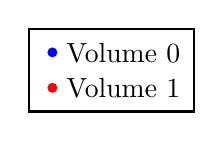
\begin{tikzpicture}[scale=0.3]
    % ... [rest of your existing TikZ picture]

    % Legend Box
    \begin{scope}[xshift=20cm, yshift=8cm]
        \draw[thick] (-1,0.5) rectangle (6,-3); % Adjusted the top border of the box
        
        \fill[blue] (0,-0.5) circle (6pt); % Blue dot
        \node[align=left] at (3,-0.5) {Volume 0}; % Moved the label to the right
        
        \fill[red] (0,-2) circle (6pt);  % Red dot
        \node[align=left] at (3,-2) {Volume 1}; % Moved the label to the right
    \end{scope}
\end{tikzpicture}
\end{frame}

\begin{frame}\frametitle{M-to-N Restarts}
\end{frame}

\begin{frame}
    \centering
    \Large
    Wrapping Up \& Looking Ahead
\end{frame}


\begin{frame}\frametitle{Summary and Next Steps}
\begin{itemize}
\item \mirgecom{} has Y3 prediction-supporting performance (poised to deliver more)
\item Understanding \mirgecom{} performance is the next major focus
\end{itemize}
\begin{center}
Next steps
\end{center}
\begin{multicols}{2}
\begin{itemize}
\item Understanding and improving performance:
\begin{itemize}
\item Instrumentation (Mem \& Tags) \prj{\tiny}{M.~Diener}
\item Code-to-kernel correspondence improvements: \prj{\tiny}{M.~Diener}
\item Auto-tuning \prj{\tiny}{Nick Christensen}
\item DAG Splat \prj{\tiny}{M. Smith}
\item Performance model
\end{itemize}
\item Upcoming enhancements:
\begin{itemize}
\item Workflow: \textit{Parsl} \prj{\tiny}{D.~Friedel}
\item Hexahedral elements \prj{\tiny}{Addison Alvey-Blanco}
\item M-to-N restart (done!)
\end{itemize}
\end{itemize}
%\columnbreak
%\end{multicols}
%\vspace{-20pt}
%\begin{center}
%  
\includegraphics[width=.48\textwidth]{Figures/mtc/Nvidia-A100-performance.eps}
%  \prj{\tiny}{Nick Christensen}
%\end{center}
\end{multicols}
\end{frame}

% - PLANS CHANGE
%\begin{frame}\frametitle{Developments for Y3 Prediction}
%\begin{center}
%Y3 Driver\\
%https://github.com/illinois-ceesd/drivers\_y3-prediction
%\end{center}
%\begin{multicols}{2}
%\begin{itemize}
%\item Kitchen sink (KS) feature set
%  \begin{itemize}
%  \item Coupled CNS + Wall/heat
%  \item Ethylene mixture, reaction sources, species limiting, power-law transport
%  \item Wall degradation, oxygen diffusion, reactive/porous mat.
%  \item Artificial physical viscosity, and sponge
%  \item OFF: Mixture transport, spectral filtering on RHS
 % \end{itemize}
%\item Meshes: 2D/3D updated geom, 2 test sects., shallower cavity
%\item Sims: 3D coupled (6M,p=4 256 GPUs), and smaller
%\item Scalability scripting and inputs (@add-scalability)
%\end{itemize}
%\end{multicols}
%\end{frame}

%\begin{frame}\frametitle{Path to Y3 Prediction}
%\begin{multicols}{2}
%\begin{itemize}
%\item Physics and modeling: Radiation \& Phenolics (mild gap)
%\item Numerics and discretization
%  \begin{itemize}
%  \item Mesh modifications (upstream injector, possible refinement)
%  \item Maybe (gaps suspected):
%    \begin{itemize}
%    \item Higher order mesh + filtering (likely!)
%    \item New AV
%    % \item Slope limiters
%    \item Multi-order meshes/volumes
%    \item ESDG? \prj{\tiny}{Zirui Wang}
%    \item Stop gap: High viscosity, maybe reduced physics
%    \end{itemize}
%  \end{itemize}
%\columnbreak
%\item Performance - closing gaps
%  \begin{itemize}
%  \item Cost per step (inert, comb): (.5, 1.4)s
%  \item Sim time: 1ms inert, 6e-4 w/comb
%  \item Estimated DT: .5ns
%  \item 12d inert, 19d comb
%  \item Any improvements welcomed
%  \end{itemize}
%\end{itemize}
%\end{multicols}
%\end{frame}

%\begin{frame}\frametitle{Path to Y3 Prediction}
%\begin{center}
%\item Preparing for prediction runs
%\end{center}
%\begin{multicols}{2}
%\begin{itemize}
%\item 3M(ish) 3D p=3 elems 
%\item Potentially serious issues: Shock/boundary, fluid/material
%\item Investigating higher order, with filtering, high visc
%\item Many scoping, physics-targeted, and debugging runs
%\end{itemize}
%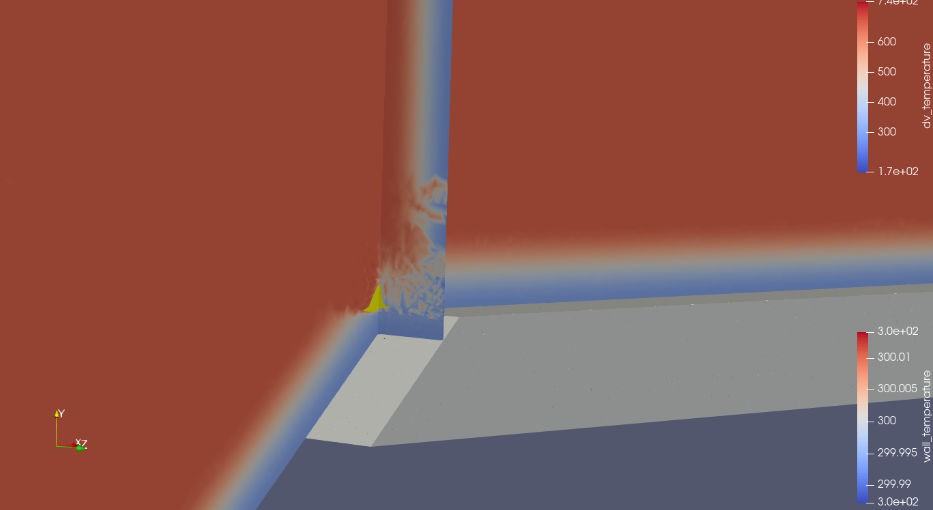
\includegraphics[width=.3\textwidth]{Figures/mtc/hot_edge.png}
%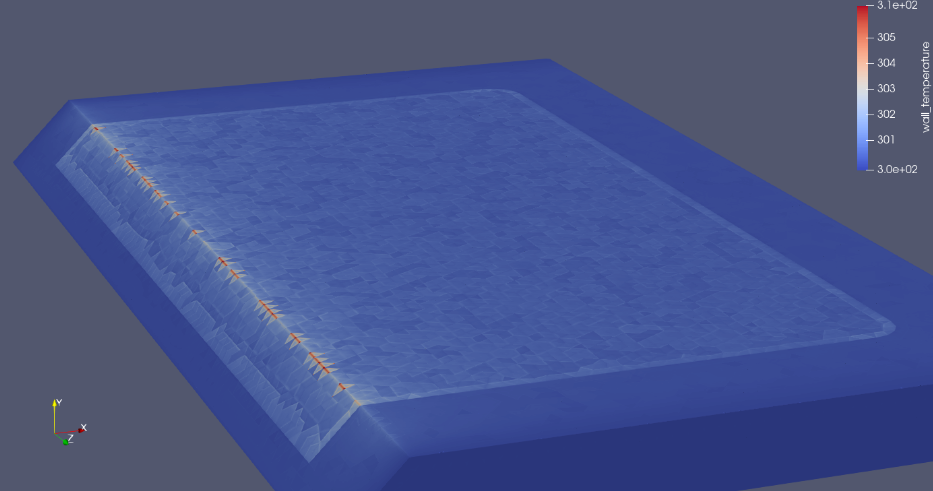
\includegraphics[width=.4\textwidth]{Figures/mtc/3d_yellow_cells.png}
%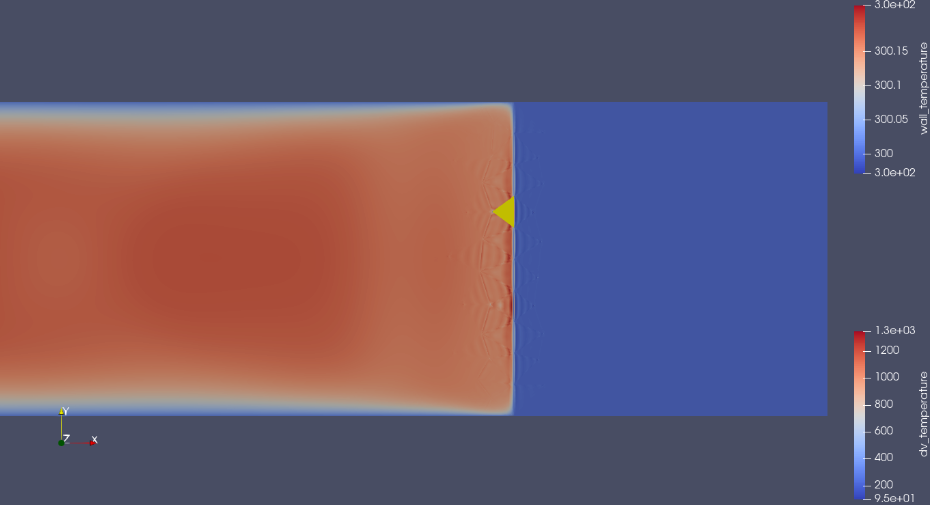
\includegraphics[width=.4\textwidth]{Figures/mtc/2d_yellow_cells.png}
%\end{multicols}
%\end{frame}

%\begin{frame}\frametitle{Path to Y3 Prediction}
%\begin{multicols}{2}
%\begin{itemize}
%\item Some pain points
%  \begin{itemize}
%  \item Transfinite or ultra fine mesh to stabilize fluid boundary
    % \begin{itemize}
    % \item Increases complexity of meshing by a lot
    % \item Increases number of elements
    % \item Hex support desired, might help
    % \end{itemize}
%  \item Lack confidence in correctness of model implementation
    % \begin{itemize}
    % \item Problem with numerics, or defect?
    % \item More extensive testing!
    % \item More experience/intuition about the numerics
    % \item ESDG?, FV?
    % \end{itemize}
%  \item Small problem performance is a drag
    % \begin{itemize}
    % \item 20m compile (this is fine, not fine)
    % \item DAG splat elim, faster compile
    % \end{itemize}
%  \item Makes lots of big files
    % \begin{itemize}
    % \item PARSL
    % \item Viz Driver
    % \end{itemize}
%  \item Development and testing viscosity
%  \item Long queues on available platforms
%  \item Cannot change size of run to adapt to resources
%  \end{itemize}
%\end{itemize}
%\end{multicols}
%\end{frame}


%\begin{frame}\frametitle{Near-term Development Outlook}
%\begin{multicols}{2}
%\begin{itemize}
%\item Now
%  \begin{itemize}
%  \item Understanding performance (why is it hard?)
%    \begin{itemize}
%    \item Code $\leftrightarrow$ Kernel \prj{\tiny}{M.~Diener}
%    \item Performance model
%    \item Kernel rooflines \prj{\tiny}{Nick Christensen}
%    \item Feature-specific
%    \end{itemize}
%  \item Evaluate Tioga
%  \item Boundary verif (MMS)
%  \item PARSL for testing \prj{\tiny}{D.~Friedel}
%  \end{itemize}
%\end{itemize}
%\columnbreak
%\begin{itemize}
%\item For prediction: (4mo horizon)
%  \begin{itemize}
%  \item Radiation \& phenolics \prj{\tiny}{T.~Ricciardi, M.~Smith}
%  \item \sout{DAG splat} \prj{\tiny}{Kaushik Kulkarni}
%  \item Mechanism parameterization for UQ
%  \item PARSL for UQ \prj{\tiny}{D.~Friedel}
%  \item Stabilizing prediction runs \prj{\tiny}{M.~Anderson}
%    \begin{itemize}
%    \item ESDG \prj{\tiny}{Zirui Wang}
%    \item Mixed-order
%    \item Quad/Hex support \prj{\tiny}{Addison Alvey-Blanco}
%    \item Curvlinear elements
%    \end{itemize}
%  \end{itemize}
%\end{itemize}
%\end{multicols}
%\end{frame}

%\begin{frame}\frametitle{Nice to have any time}
%\begin{multicols}{2}
%\begin{itemize}
%\item Reducing prediction pain (important):
%  \begin{itemize}
%  \item Reduce technical debt (merges)
%  \item Driver unification
%  \item Help with mesh generation
%  \item Visualization driver
%  \item PARSL for queue management
%  \item M-to-N restart
 % \end{itemize}
%%\item Potentially high-impact performance improvements
%  \begin{itemize}
%  \item Kernel Autotuning \prj{\tiny}{Nick Christensen}
%  \item Node-aware communication \prj{\tiny}{Shelby Lockhart}
%  \item DAG/compile time improvements \prj{\tiny}{Kaushik Kulkarni, M.~Diener}
%  \item Instrumentation (Mem \& Tags) \prj{\tiny}{Kaushik Kulkarni, M.~Diener}
%  \end{itemize}
%\item Future sims
%  \begin{itemize}
%  \item Mesh motion (interface regression)
%  \item Wall degradation
%  \item Turbulence modeling
%  \end{itemize}
%\end{itemize}
%\end{multicols}
%\end{frame}


\begin{frame}[fragile]\frametitle{Create the DG Discretization (4/7)\prj{\tiny}{M.~Smith}}

\vspace{-1.1in}

\begin{itemize}
\item Create a DG discretization on each of the elements in the mesh 
\item Represented by a {\color{myOrange}\texttt{DiscretizationCollection}} which
  contains sub-discretizations for all mesh entities (volume, interior faces, boundaries,
  etc.)
\end{itemize}

\begin{tikzpicture}[overlay,remember picture]
\node(code)at([yshift=-0.5in]current page.center){
  \begin{minipage}{0.9\textwidth}
    \begin{lstlisting}[style=mintedlike,basicstyle=\mintedlikebasicstyle{\footnotesize}]
  from mirgecom.discretization import create_discretization_collection
  dcoll = create_discretization_collection(actx, local_mesh, order=3)

  # nodes() without an argument returns volume nodes on the base discretization
  nodes = actx.thaw(dcoll.nodes())

  # Used in operator calls if running with overintegration
  if use_overintegration:
      from grudge.dof_desc import DISCR_TAG_QUAD
      quadrature_tag = DISCR_TAG_QUAD
  else:
      quadrature_tag = None
    \end{lstlisting}
  \end{minipage}
};
\end{tikzpicture}

\end{frame}

\begin{frame}[fragile]\frametitle{Visualization, Restart, and Logging\prj{\tiny}{M.~Smith}}

\begin{itemize}
\item {\large\cPI{Visualization}}
  \begin{itemize}
  \normalsize
  \item Output as parallel VTK files, which can be read by ParaView
  \item Support arbitrary viz. fields
  \end{itemize}
\item {\large\cPI{Restart}}
  \begin{itemize}
  \normalsize
  \item Restart data is serialized via \textit{pickle} and written to a
    separate file for each MPI rank
  \item {\color{myOrange}New for Y3:} Partition remapping (``M-to-N'') functionality \prj{\tiny}{M.~Campbell}
  \end{itemize}
\item {\large\cPI{Logging}}
  \begin{itemize}
  \normalsize
  \item Logging functionality provided by \textit{logpyle} package \prj{\tiny}{M.~Diener}
  \item Writes status output to terminal and additional output to database files
  \item Tracks state quantities as well as profiling data
  \end{itemize}
\end{itemize}
\end{frame}

\begin{frame}[fragile]\frametitle{Tensor Product Element Timings}

  \begin{itemize}
  \item Nascent support for tensor-product elements (TPE) [Quads and Hexes]
  \item Initial tests in \textit{mirgecom} ACTII pass physics tests, but performance is prohibitive
  \item Testing improvements... more data real soon
  \end{itemize}
\begin{table}
\centering
\begin{tabular}{|l|c|c|c|c|}
\hline
\multirow{2}{*}{Test Case} & \multicolumn{2}{c|}{Compile Time (s)} & \multicolumn{2}{c|}{Step Time (s)} \\ \cline{2-5} 
                           & T       & Q      & T       & Q       \\ \hline
Smoke Test 2D (Single Gas) & 40.3    & 225.8  & 0.044   & 0.11    \\ \hline
Smoke Test KS (Mixture)    & 47.0    & 2372.2 & 0.91    & 11.6    \\ \hline
KS w/(AV+Wall) OFF         & 105.6   & 505.4  & 0.89    & 6.7     \\ \hline
\end{tabular}
\caption{Compilation and Simulation Step Times for 2D Finite Elements (T for Triangles, Q for Quads)}
\end{table}

\end{frame}
